\documentclass[a4paper,10pt]{article}
\usepackage[french]{babel} 
\usepackage[utf8x]{inputenc}
\usepackage[T1]{fontenc}
\usepackage{lmodern}
\usepackage{makeidx}
\usepackage{multicol}
\usepackage{hyperref}
\usepackage{pdfpages}

\newcommand{\etal}{\textit{et al.}}

\title{
  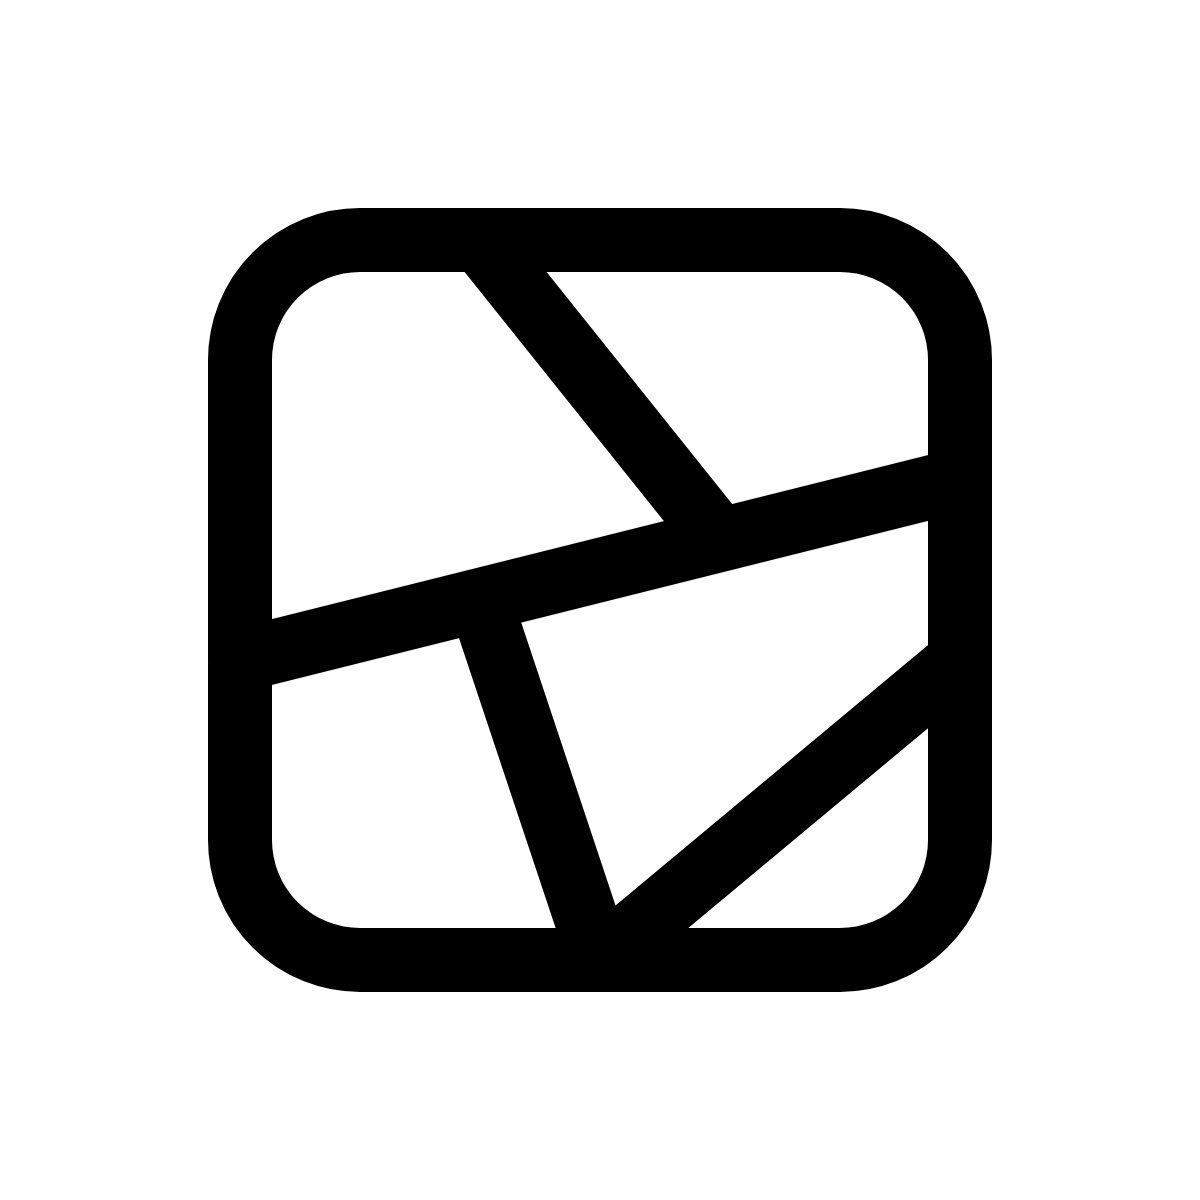
\includegraphics[width=2cm]{../iconography/phragment-black.png}\\
  \bsc{Phragment}\\
  \large{
    Une tentative protocole pour des conversations décentralisées
    où tout le monde est propriétaire de son contenu\\~\\~\\
    \textbf{version} \texttt{0.0.1}
  }
}

\date{}
\author{
  Xavier \bsc{Van de Woestyne}\\
  \texttt{xaviervdw@gmail.com}\\
  \small{https://xvw.github.io}
}


\hypersetup{ hidelinks, }
\addto{\captionsfrench}{\renewcommand{\abstractname}{}}

\begin{document}

\maketitle

\begin{abstract}
  A l'heure ou le web décentralisé revient à la tendance, pour de multiples
  raisons valables (écologiques, morales et idéologiques, ouvertures de
  perspectives), on trouve beaucoup de solutions qui pallient à des soucis
  liés à l'excès de centralisation dans le web. \bsc{Phragment} est un
  protocole dont l'objectif initial est de servir un système de commentaires
  pour une application web statique, tâchant de permettre aux intervenants
  de contrôler leurs différents contenus. Le protocole ne décrit aucune
  innovations particulières et souffre d'un manque d'ergonomie flagrant,
  cependant, j'assume parfaitement le plaisir de réinventer, encore une fois,
  une roule, bancale et peu robust. L'objectif de ce document est de survoler
  les motivations (et le contexte) d'un tel protocol, son formalisme,
  l'élaboration d'un client de référence, le survol de certains cas d'usages,
  les améliorations possibles, points de blocages et faiblesses intrinsèques.
\end{abstract}


\newpage
\bibliographystyle{unsrt}
\bibliography{phragment.bib}

\end{document}
